\documentclass{article}%
\usepackage[T1]{fontenc}%
\usepackage[utf8]{inputenc}%
\usepackage{lmodern}%
\usepackage{textcomp}%
\usepackage{lastpage}%
\usepackage[head=40pt,margin=0.5in,bottom=0.6in]{geometry}%
\usepackage{graphicx}%
%
\title{\textbf{Entrevista a Carleth Morales: “La resistencia no está muerta”}}%
\author{Annie van Der Dyst}%
\date{17/11/2018}%
%
\begin{document}%
\normalsize%
\maketitle%
\textbf{URL: }%
http://www.el{-}nacional.com/noticias/papel{-}literario/entrevista{-}carleth{-}morales{-}resistencia{-}esta{-}muerta\_259968\newline%
%
\textbf{Periodico: }%
EN, %
ID: %
259968, %
Seccion: %
Papel Literario\newline%
%
\textbf{Palabras Claves: }%
Papel Literario\newline%
%
\textbf{Derecho: }%
CONTEXTO%
, Otros Derechos: %
12%
, Sub Derechos: %
NO\_TIENE%
\newline%
%
\textbf{EP: }%
NO\newline%
\newline%
%
\textbf{\textit{Carleth Morales es periodista y autora de “26 crímenes y una crónica. ¿Quién mató a la resistencia venezolana?”}}%
\newline%
\newline%
%
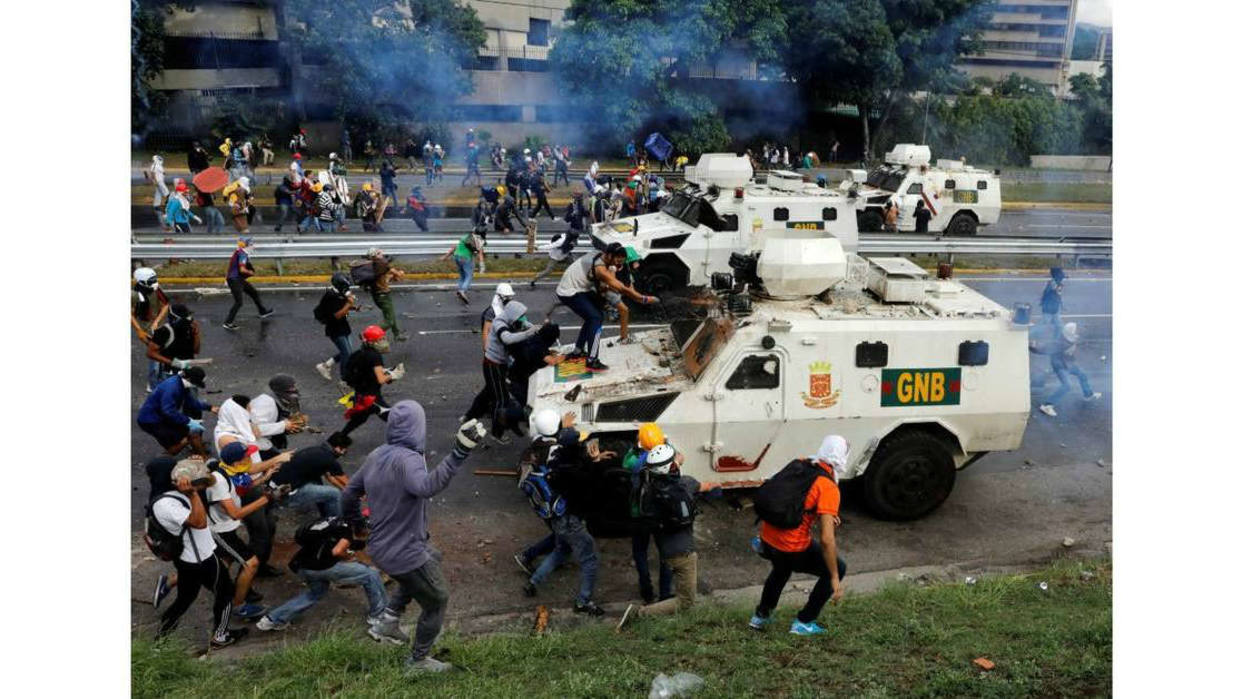
\includegraphics[width=300px]{210.jpg}%
\newline%
%
\&horbar;¿Primavera venezolana?%
\newline%
%
“Si consultamos Wikipedia esta nos refiere que la ola de protestas que sacudió a Venezuela en el año 2017, especialmente entre los meses de abril y agosto, fue una ola de manifestaciones populares a nivel nacional e internacional que buscaban una salida democrática a la crisis institucional y a otros eventos relacionados con la conflictividad política del país, especialmente a raíz de las elecciones parlamentarias del 2015. El objeto de esas protestas era pedir elecciones para la revocación del mandato del presidente Nicolás Maduro.%
\newline%
%
Los medios de comunicación hablaron de la ‘Primavera venezolana’ o la ‘Rebelión de abril’”.%
\newline%
%
\&horbar;Otras primaveras.%
\newline%
%
“La ‘Primavera de Praga’ fue un periodo de liberación política en Checoslovaquia ocurrido durante la Guerra Fría que se prolongó desde el 5 de enero hasta el 20 de agosto cuando el país fue invadido por la URRSS y sus aliados de Varsovia.%
\newline%
%
Más cercana en el tiempo, la ‘Primavera árabe’ también fue un conjunto de manifestaciones populares que sacudieron a varios países de la región, un clamor por la democracia y los derechos sociales organizado por la población árabe. Más largo y complejo es hablar de los resultados de estas protestas populares (donde tanto ha tenido que ver la intervención extranjera), la creación del Estado Islámico y la sangrienta e inacabable guerra siria son algunas de sus consecuencias”.%
\newline%
%
\&horbar;¿Cuáles fueron las consecuencias de la Primavera venezolana?%
\newline%
%
“El Foro Penal Venezolano reseña que el 2017 fue un año récord en la represión venezolana: desde el 1º de enero al 31 de diciembre se registraron 5.511 arrestos con fines políticos, la mayoría producidos entre abril y agosto. La mencionada organización señala un aumento del 1.200 \% en comparación al total de las cifras de 2016 cuando se registraron 69 casos de presos políticos.%
\newline%
%
Son cifras que hablan de la represión por parte de las autoridades estatales y que dejaron un saldo de 158 víctimas mortales y, al parecer, una población derrotada que concentra sus esfuerzos en huir de un país que se ha quedado, también, sin la palabra esperanza”.%
\newline%
%
\&horbar;¿Cuál es la conclusión a la que llega usted después del arduo proceso de investigación y entrevistas, quién mató a la resistencia venezolana?%
\newline%
%
“Lo primero que hay que decir es que la resistencia no está muerta, puede parecer una contradicción dado el subtítulo del libro, pero no lo es. Realmente la pregunta busca respuestas en varios escenarios. El primero, por supuesto, plantea la necesidad de saber quién o quiénes mataron a las 158 personas que señalan las estadísticas extraoficiales como víctimas de las protestas de 2017, la mayoría jóvenes, muchachos asesinados por ejercer su derecho a la protesta, y en la búsqueda de esa respuesta tenemos que involucrarnos todos, no solo los padres, porque la justicia se antoja necesaria, prioritaria y necesaria. Y a partir de allí, el resto de escenarios hacia los que apunta la interrogante es, entre otros, a nosotros mismos: ¿qué nos pasa?, ¿no somos capaces de reaccionar?, ¿nuestra capacidad de enfrentarnos a este nefasto gobierno está muerta? Si hay algo que es tan cierto como que esos jóvenes están enterrados, es que nuestra inacción los va a seguir matando, a ellos y a nosotros”.%
\newline%
%
\&horbar;¿Hay posibilidades de que se reactive la resistencia en las circunstancias actuales?%
\newline%
%
“En 2017 la mayoría de los venezolanos creía en la dirigencia política de oposición, y lo hizo durante cuatro meses seguidos, incluso, cada día con más fuerza, pero instaurada la Asamblea Nacional Constituyente y en virtud de que intentando evitarla y restituir el hilo democrático asesinaron a más de un centenar de jóvenes, está claro que la salida deliberada a la calle no está planteada en este momento, al menos no como una acción que obedezca a un llamado de un dirigente o tolda política. La resistencia está activa de otra manera, de una u otra forma, todos estamos en resistencia”.%
\newline%
%
\&horbar;Según se desprende de la lectura del libro tanto la represión encabezada por Nicolás Maduro, cuyas órdenes fueron claramente disparar a matar, como la actitud de la oposición, de seguir llamando a la toma de las calles cuando era claro que no podían impedir los asesinatos, se concatenaron para alcanzar la alta cifra de muertes durante las manifestaciones del 2017. ¿Cómo se llega a tal capacidad de pasar por encima de los derechos humanos por parte de un estado democrático?%
\newline%
%
“Lo primero que tenemos que tener claro es que Venezuela no es un Estado democrático sino una dictadura revestida de democracia, que en la teoría se vale de unas elecciones para, en la práctica, actuar como un régimen totalitario, violando todas las libertades y concentrando el poder en una persona o un grupo de ellas. En ese contexto ningún Estado ha respetado nunca los derechos humanos y, lo que es peor, los viola y hace que parezca que los han violado otros”.%
\newline%
%
\&horbar;¿Cómo los partidos de la oposición olvidan al poco tiempo, o inmediatamente, a sus muertos y son incapaces de pedir justicia para ellos?%
\newline%
%
“Los partidos de oposición no han estado a la altura de las circunstancias, les ha faltado amplitud de miras, estrategia, una verdadera unión. Seguimos pensando que estamos ante un Estado democrático, como decíamos hace un momento, y no es así. En consecuencia, todas las acciones que emprenden van en este sentido pero terminan estando a la zaga del totalitarismo. El día que se adelanten a las previsibles y –en la mayoría– anunciadas acciones del régimen totalitario, podrán recuperar parte de la credibilidad que perdieron tras la instalación de la Asamblea Nacional Constituyente”.%
\newline%
%
\&horbar;¿Es posible que esa dirigencia pueda construir de nuevo un país?%
\newline%
%
“No solo es posible, es imperativo, pero debe pensar en perspectiva, terminar de una vez por todas de aprender de sus errores, desarrollar estrategias y despojarse de las individualidades, ya habrá tiempo para lucir los egos, antes hay que recuperar la democracia”.%
\newline%
%
\&horbar;¿Cambió su perspectiva del conflicto político en Venezuela después de escribir el libro?%
\newline%
%
“Cambiaron muchas cosas, pero la perspectiva del conflicto político no. Seguimos teniendo un monstruo que se hace cada vez más grande y una dirigencia opositora que se hace cada vez más pequeña. Se ha incrementado la tragedia, pero el problema de fondo sigue siendo el mismo”.%
\newline%
%
\&horbar;¿Hay un antes y un después para Carleth Morales Senges?%
\newline%
%
“Hay un antes y un después para los padres y hermanos de los asesinados. Para mí, lo que hay es una necesidad de hacer visible su dolor para salvarlos a ellos del olvido y a nosotros de la indolencia. Si algo ha cambiado en mí, es mi percepción de las prioridades”.%
\newline%
%
\&horbar;¿Qué la inspiró a escribir este libro?%
\newline%
%
“Como periodista, me inspiró la necesidad de dejar impresa una investigación seria sobre este capítulo de nuestra historia, para no olvidar, para dejar una crónica detallada que aporte pistas a futuros estudios, y en eso tengo que agradecer el arrojo de mi editor, Sergio Dahbar, y la dedicación de mi equipo: Ashley Flores y Luis Fernando Herrera. Como venezolana, me inspiró la necesidad de denunciar ante los organismos internacionales que velan por los derechos humanos la presencia de un patrón sistemático en la actuación de las fuerzas de seguridad del Estado contra los manifestantes. Como madre, me inspiró la necesidad de escuchar y solidarizarme con los padres de las víctimas mortales, que luchan solos contra la iniquidad y el olvido”.%
\newline%
%
\&horbar;¿Hubo algún trabajo periodístico anterior que le sirvió de musa –trabajos de otros periodistas– a la hora de elaborar el formato de preguntas, la selección de los 26 casos, así como el andamiaje de cada caso? Me parece muy interesante y efectiva la estructura que mezcla el tono periodístico: los datos apegados a la realidad con las voces de familiares de las víctimas. Esta estructura transforma la lectura en un relato emocional sobre la vida de estos jóvenes cuyo clímax alcanza el final con los fríos datos y cifras del puesto que ocupan en el número de muertos por la violencia política en el país. Y como estocada, la sonriente y esperanzadora foto de los muchachos asesinados, acompañada de una frase de su autoría, llena de esperanza por un futuro. Es inevitable para el lector el sentimiento de dolor, ira e impotencia.%
\newline%
%
“No, y lo hice de forma deliberada, no quise leer nada que estuviese escrito anteriormente sobre ello para no contaminar la investigación, para que fuese lo más objetiva y limpia posible. El formato de preguntas lo elaboré con la intención de responder las interrogantes que –como te comentaba anteriormente– me hacía como periodista, venezolana y madre. Trabajar con unos padres a los que les han asesinado a su hijo por pensar diferente, te hace ser absolutamente impecable en las formas y en el tratamiento de la información, es un elemento humano que en periodismo te hace trabajar al filo del amarillismo y la interpretación, y eso no me lo podía permitir. Aunque entrevistas hice más de 50, si al final fueron 26 los testimonios de familiares y no 158, fue por tiempo y circunstancias, no por otro factor. Yo estoy a siete mil kilómetros de las fuentes y mi equipo en Venezuela también se enfrenta a la falta de luz, Internet y otras carencias. Pedí y pido perdón a los familiares a los que no pudimos llegar, pero estoy convencida de que la estructura del libro los recuerda a todos”.%
\newline%
%
\&horbar;En muchos casos llama la atención que se repiten algunas características, la condición de hijos únicos o hijos de madres solteras, jóvenes que apenas alcanzaban los veinte años, sin militancia en ningún partido político y sin pertenencia a organizaciones anti gubernamentales. ¿Qué conclusión saca usted de estos datos?%
\newline%
%
“Es difícil afirmar que fueron escogidos por los cuerpos de seguridad, que los tenían identificados y que sabían a quiénes iba a disparar y a quiénes no. Es posible, pero como periodista eso no lo puedo dar por cierto. Yo lo atribuyo más a otro factor y es que quienes estaban al frente de las protestas eran los jóvenes fuertes, los que comían porque sus padres luchaban cada día por sacarlos adelante en vez de estar esperando una bolsa del CLAP; los que estudiaban en una universidad y sabían el valor del esfuerzo y la constancia en vez de estar esperando que alguien los enchufara para darles un cupo; los que no le debían nada al gobierno; los que escuchaban a sus padres contar cómo era la Venezuela en la que ellos habían crecido a base de esfuerzo y trabajo; los que leían, escribían, reflexionaban y creían en una Venezuela construida sobre la base de los valores que veían en sus casas. Por eso tenían todos el mismo perfil, por eso, cuando un guardia disparaba contra uno, daba igual si disparaba contra el de al lado. Todos eran iguales”.%
\newline%
%
\&horbar;¿Cuál es la resistencia que existía en el país?%
\newline%
%
“La que existía y la que sigue existiendo: jóvenes con valores, personas de todas las edades educadas en valores. Porque si bien es cierto que asesinaron a unos, los que siguen vivos volverán a salir y serán los que den la cara, en cualquier escenario, para salvar a Venezuela”.%
\newline%
%
\&horbar;¿Tendrá ahora las misma características?%
\newline%
%
“Después de las protestas de 2017, el país no es el mismo, definitivamente. Si algo hemos aprendido es que el régimen está armado y no le tiembla el pulso a la hora de disparar”.%
\newline%
%
\&horbar;Al parecer las manifestaciones y protestas del 2017 no han tenido ningún efecto desestabilizador del gobierno de Nicolás Maduro. ¿Cree usted que aún hay jóvenes dispuestos a protestar en Venezuela?%
\newline%
%
“La Constituyente fue un instrumento que sacó Nicolás Maduro y su equipo después de un mes de protestas, cuando vio que no tenía otra forma de apagar la calle y acallar el clamor de la comunidad internacional sobre el autogolpe, tras arrebatarle las funciones al legislativo legítimo. En ese sentido sí tuvieron su efecto desestabilizador, pero como dije al comienzo, la oposición no supo tomar la delantera y continuó a la zaga, protestando a partir de mayo por algo que en abril, cuando comenzaron las protestas, no existía. El gobierno se vio obligado a jugarse esa carta, que ha acabado siendo el suprapoder contra el que nadie ha podido luchar, ni siquiera los jóvenes desarmados que querían un país mejor. Pero eso no quiere decir que no estén dispuestos a protestar, el problema es que está demostrado que si lo hacen a pecho descubierto en una calle los pueden matar, sin más, y después meter su expediente en el cajón de la Fiscalía, o del olvido, que es lo mismo. Lo harán de otra manera, pero lo harán”.%
\newline%
%
\&horbar;Como periodista ¿cómo contribuye su libro en la búsqueda de justicia para las víctimas y sus familiares?%
\newline%
%
“Yo no soy abogado ni juez, con lo cual obrar justicia no está en mis manos. Yo soy periodista y lo que puedo hacer es ruido, que es lo que estoy haciendo. Este libro es una investigación que estoy consignando ante los organismos internacionales para que, de alguna manera, sean también tomados en cuenta estos casos a la hora de contemplar la posibilidad de aplicar sanciones a los responsables de estos crímenes y aplicar sobre ellos los convenios internacionales a los que hubiere lugar. En todo caso, la justicia legal llegará, pero mientras llega, la justicia moral ya los ha condenado”.%
\newline%
%
\&horbar;Háblenos un poco de las distintas presentaciones del libro en ámbitos internacionales y la acogida que han dado organismos de defensa de los derechos humanos a las historias que en él se cuentan.%
\newline%
%
“El libro lo presenté por primera vez el 26 de abril, en Ginebra, ante la Oficia del Alto Comisionado por los Derechos Humanos de la ONU, donde la Alta Comisionada Adjunta, Kate Gilmore, lo recibió y me agradeció el hecho de haber investigado y presentado el trabajo personalmente allí. ‘Agradezco el esfuerzo y será tomado en cuenta’, me dijo. También lo presenté ante la Subcomisión de Derechos Humanos del Parlamento Europeo, donde su vicepresidenta, Beatriz Becerra, abrió las puertas de la sede en Madrid para acoger un acto con los familiares de las víctimas. El libro ha recorrido instituciones en España como el Congreso, el Senado, la Diputación de Guipúzcoa y otras interesadas en conocer su contenido. En todos los casos hay mucha sensibilidad hacia la tragedia que vive Venezuela y eso es positivo, porque se traduce en pronunciamientos y sanciones, que al final también es el objetivo”.%
\newline%
%
\&horbar;Después de visualizar el doloroso resultado de las protestas masivas del 2017, las elecciones de Maduro, su permanencia en el poder, la falta de justicia con respecto a las víctimas de los homicidios en las manifestaciones, ¿cree usted que el país está preparado para conseguir un cambio que haga posible la salida de Maduro del poder?%
\newline%
%
“El país, más que preparado, lo que está es ávido de un cambio. Cada hora que pasa aumenta la escasez, la desnutrición, el hambre, la falta de medicamentos, de acceso a la salud, a la justicia, a lo más básico que es la vida. Y eso no es bloqueo, eso es ineptitud y la evidencia de un modelo de gobierno fracasado que tiene que cambiar cuanto antes. Los venezolanos no aguantamos más. Hay muchos grupos y organizaciones que, desde la diáspora, están trabajando en la transición, lo único que tiene que suceder para reconstruir a Venezuela es que este gobierno caiga”.%
\newline%
%
\end{document}